\documentclass{article}

\usepackage{url}
\usepackage{amsmath,amssymb}
\usepackage{graphicx,svg}

\begin{document}
\title{Lecture 11\\ Properties of Laplace Transform}
\author{C.L. Wyatt}
\date{\today}
\maketitle

Last week we learned how to compute the forward Laplace transform and Inverse Laplace transform for causal signals using the integrals


$$
\begin{aligned}
X(s)=\int\limits_{0}^{\infty} x(t) e^{-s t}\; dt \quad\text{and}\quad x(t)=\frac{1}{2 \pi j} \int\limits_{c- j \infty}^{c+j \infty} X(s) e^{s t}\; ds
\end{aligned}
$$

Today we will go over several usefully properties of these transforms, that when combined with a table of transforms will allow us to analyze wide variety of stable and unstable systems.

Note: unless otherwise specified, in the following the Laplace transforms are one-sided (unilateral).

\section{Linearity Property}

For $X_{1}(s)=\mathcal{L}\left\{x_{1}(t)\right\}$ and $X_{2}(s)=\mathcal{L}\left\{x_{2}(t)\right\}$

$$
\mathcal{L}\left\{a x_{1}(t)+b y_{2}(t)\right\}=a X_{1}(s)+b X_{2}(s)
$$
for $a, b \in \mathbb{C}$

\subsection{Proof}

$$
\begin{aligned}
\mathcal{L}\left\{a x_{1}(t)+b x_{2}(t)\right\} & =\int_{0}^{\infty}\left(a x_{1}(t)+b x_{2}(t)\right) e^{-s t} d t \\
& =a \int_{0}^{\infty} x_{1}(t) e^{-s t} d t+b \int_{-\infty}^{\infty} x_{2}(t) e^{-s t} d t \\
& =a X_{1}(s)+b X_{2}(s)
\end{aligned}
$$

\subsection{Example 11.1}
If $x(t)=4 e^{-t} u(t)-7 e^{-5 t} u(t) \quad X(s)=$ ?

$$
\begin{aligned}
\mathcal{L}\{x(t)\} & =\mathcal{L}\left\{4 e^{-t} u(t)-7 e^{-5 t} u(t)\right\} \\
& =4 \mathcal{L}\left\{e^{-t} u(t)\right\}-7\mathcal{L}\left\{e^{-5 t} u(t)\right\} \\
& =\frac{4}{s+1}+\frac{-7}{s+5}
\end{aligned}
$$

\subsection{Example 11.2}

This also works in reverse. If $X(s)=\frac{10}{s+2}+\frac{3}{s+10}=\frac{13 s+106}{s^{2}+12 s+20}$

$$
\begin{aligned}
x(t)=\mathcal{L}^{-1}\left\{\frac{10}{s+2}+\frac{3}{s+10}\right\} & =10 \mathcal{L}^{-1}\left\{\frac{1}{s+2}\right\}+3 \mathcal{L}^{-1}\left\{\frac{1}{s+10}\right\} \\
& =10 e^{-2 t} u(t)+3 e^{-10 t} u(t)
\end{aligned}
$$

\section{Time Shift Property}

For causal $x(t)$ with $X(s) = \mathcal{L}\left\{x(t)\right\}$, then for time delay $t_0 \geq 0$

\[
\mathcal{L}\left\{ x(t-t_0) \right\} = X(s) e^{-s t_0}
\]

Note, in general, the time shift can only be a delay since an advance could make the signal non-causal. A more complete definition would be that as long as the time shift does not cause the signal to become non-causal.

\subsection{Proof}

\[
\mathcal{L}\left\{x\left(t-t_{0}\right)\right\} =\int_{0}^{\infty} x\left(t-t_{0}\right) e^{-s t} \; dt
\]

Let $\tau = t-t_0$, then $t = \tau + t_0$ and $d\tau = dt$, thus

$$
\begin{aligned}
\mathcal{L}\left\{x\left(t-t_{0}\right)\right\} &= \int_{t_{0}}^{\infty} x(\tau) e^{-s\left(\tau+t_{0}\right)} d\tau\\
& =\int_{0}^{\infty} x(\tau) e^{-s \tau} e^{-s t_{0}} \; d\tau = e^{-s t_{0}} X(s)
\end{aligned}
$$

\subsection{Example 11.3}

Let $x(t)=v(t)=v(t-10)$, a causal pulse of 10 seconds.

$$
\begin{aligned}
\mathcal{L}\{x(t)\} & =\mathcal{L}\{u(t)-u(t-10)\} & & \\
& =\mathcal{L}\{u(t)\}-\mathcal{L}\{u(t-10)\} & & \text { by linearity property } \\
& =\frac{1}{5}-\frac{1}{5} e^{-10s} & & \text { by time-shift property. }
\end{aligned}
$$


\subsection{Example 11.4}

When doing inverse transforms, collect all terms with common shift and do PFE separately in each. For example let

\[
X(s)=\frac{e^{-7 s} s^2 + \left(e^{-4s} + 3e^{-7s}\right)s + \left(4e^{-4s} + 2e^{-7s} \right)}{(s+4)\left(s^{2}+3 s+2\right)}
\]

First rewrite in terms of the delays:

\[
X(s)=\frac{e^{-4 s}(s+4)+e^{-7 s}\left(s^{2}+3s+2\right)}{(s+4)\left(s^{2}+3 s+2\right)}
\]

Then separate and take the inverse of each term independently, e.g.

$$
\begin{aligned}
& =\frac{e^{-4 s}}{s^{2}+3s+2}+\frac{e^{-7 s}}{s+4} \\
& =e^{-4 s}\left[\frac{k_{1}}{s+1}+\frac{k_{2}}{s+2}\right]+e^{-7 s}\left[\frac{1}{s+4}\right] \\
& =e^{-4 s}\left[\frac{1}{s+1}+\frac{-1}{s+2}\right]+e^{-7 s}\left[\frac{1}{s+4}\right] \\
x(t) & =\left[e^{-t} u(t)-e^{-2 t} u(t)\right]_{t\rightarrow t-4} + \left[e^{-4 t} u(t)\right]_{t\rightarrow t-7} \\
& =e^{-(t-4)} u(t-4)-e^{-2(t-4)} u(t-4)+e^{-4(t-7)} u(t-7)
\end{aligned}
$$

\section{Frequency Shift}

Consider a causal signal $f(t)$ with Laplace transform $F(s)$. Let $x(t)=f(t) e^{s_{0} t}$ for $s_{0} \in \mathbb{C}$

Then

\[
\mathcal{L}\{x(t)\}=F\left(s-s_{0}\right)=\left.F(s)\right|_{s \rightarrow s-s_{0}}
\]

The proof is a bonus problem on this week's problem set.

\subsection{Example 11.5}

$x(t)=\cos \left(\omega_{0} t\right) u(t) \quad \omega_{0} \in \mathbb{R}, \quad x(s)=$ ?

$$
\begin{aligned}
x(t) & =\frac{1}{2} e^{j \omega_{0} t} u(t)+\frac{1}{2} e^{-j \omega_{0} t} u(t) \quad \text { by Eulers } \\
\mathcal{L}\{x(t)\} & =\frac{1}{2} y\left\{e^{j \omega_{0} t} u(t)\right\}+\frac{1}{2} y\left\{e^{-j \omega_{0} t} u(t)\right\} \text { by linearity } \\
& =\left.\frac{1}{2} \mathcal{L}\{u(t)\}\right|_{s \rightarrow s-j \omega_{0}}+\left.\frac{1}{2} \mathcal{L}\{u(t)\}\right|_{s \rightarrow s + j\omega_{0}} \\
& =\frac{1}{2} \frac{1}{s-j \omega_{0}}+\frac{1}{2} \frac{1}{s+j \omega_{0}} \\
& =\frac{1}{2}\left[\frac{s+j \omega_{0}+s-j \omega_{0}}{\left(s-j \omega_{0}\right)\left(s+j \omega_{0}\right.}\right] \\
& =\frac{1}{2}\left[\frac{2 s}{s^{2}+\omega_{0}^{2}}\right]=\frac{s}{s^{2}+\omega_{0}^{2}}
\end{aligned}
$$

\section{Time Differentiation}

Let $X(s)=\mathcal{L}\{x(t)\}$ then

$$
\mathcal{L}\left\{\frac{d x}{d t}\right\} \text { for } t \geq 0 \text { is } s X(s)-x\left(0^{-}\right)
$$
where $x\left(0^{-}\right)$ is the signal value at $t=0^{-}$, which for a causal signal is zero. Repeated differentiation gives general form

$$
\mathcal{L}\left\{\frac{d^{n} x}{d t^{n}}\right\}=\left. s^{n} X(s)-\sum\limits_{k=1}^{n} s^{n-k} \frac{d^{k-1}}{d t^{k-1}} x(t) \right|_{t=0^{-}}
$$

We will discuss this property in detail with examples when we cover solving LCCDE next time.

\section{Frequency Differentiation}

Let $x(t) \stackrel{\mathcal{L}}{\longleftrightarrow} X(s)$, then 


$$
-t x(t) \stackrel{\mathcal{L}}{\longleftrightarrow} \frac{d X(s)}{d s}
$$

Note this is complex differentiation as described in lecture 7.

\subsection{Example 11.6}

Find $\mathcal{L}\{t u(t)\}$, the ramp signal.

$$
\begin{aligned}
\mathcal{L}\{t u(t)\} & =-\mathcal{L}\{-t u(t)\}=-\frac{d X(s)}{d s} \text { where } X(s) =\mathcal{L}\{u(t)\} =\frac{1}{s}\\
& =-\frac{-1}{s^{2}}=\frac{1}{s^{2}}
\end{aligned}
$$

\section{Integration Property}

Let $x(t) \stackrel{\mathcal{L}}{\longleftrightarrow} X(s)$, then 

$$
\int\limits_{0^-}^t  x(\tau) \; d\tau \stackrel{\mathcal{L}}{\longleftrightarrow} \frac{X(s)}{s}
$$

\subsection{Example 11.7}

Recall the integrator block

\begin{figure}
  \centering
  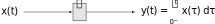
\includegraphics[alt={integrator block. See caption.}]{figures/fig11_1.svg}
  \caption{The integrator block in the time domain. It computes the running integral of its input and is a building block for CT systems.}
\end{figure}

Taking the Laplace transform of input and output and assuming a causal input (zero initial conditions for non-input nodes)

\[
Y(s) = \frac{1}{s} X(s) \quad .
\]

This is why the integrator block is often depicted as

\begin{figure}
  \centering
  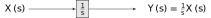
\includegraphics[alt={integrator block in Laplace domain. See caption.}]{figures/fig11_2.svg}
  \caption{The integrator block in the Laplace domain.}
\end{figure}

\section{Time Scaling Property}

Given $x(t) \stackrel{\mathcal{L}}{\longleftrightarrow} X(s)$. For $a>0$

$$
\mathcal{L}\{x(a t)\} \longleftrightarrow \frac{1}{a} X\left(\frac{s}{a}\right)
$$

Recall this corresponds to speeding up or slowing down a signal.

\section{Time Convolution}

Let $x_{1}(t) \stackrel{\mathcal{L}}{\longleftrightarrow} X_{1}(s)$ and $x_{2}(t) \stackrel{\mathcal{L}}{\longleftrightarrow} X_{2}(s)$ then

$$
x_{1}(t) * x_{2}(t) \stackrel{\mathcal{L}}{\longleftrightarrow} X_{1}(s)\cdot X_{2}(s)
$$

So for causal systems with impulse response $h(t)$, the output in the Laplace domain is

$$
Y(s)=H(s) X(s) \text { where } H(s)=\mathcal{L}\{h(t)\} \text { and } X(s)=\mathcal{L}\{x(t)\}
$$

To get $y(t)=\mathcal{L}^{-1}\{Y(s)\}$. Recall $H(s)$ is transfer function. This implies $H(s)=\frac{Y(s)}{X(s)}$

This gives us an analysis approach similar to how the Fourier transform was used in ECE 2714, except now it works for unstable systems.

\begin{figure}
  \centering
  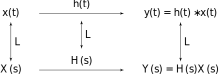
\includegraphics[alt={illustration of analysis approach using Laplace. See caption.}]{figures/fig11_3.svg}
  \caption{Illustration of the various CT LTI systems analysis methods using Laplace.}
\end{figure}

\subsection{Example 11.8}

Suppose we have a first order LTI System with $h(t)=3 e^{-2 t} u(t)$ with input $x(t)=\cos (10 t) u(t)$. Find $Y(s)$ and $y(t)$ using Laplace.

\textbf{Solution:}

\begin{itemize}
  \item We note $H(s)=\mathcal{L}\left\{3 e^{-2 t} u(t)\right\}=\frac{3}{s+2}$ (linearity + table)
  \item From table (or proved earlier) $X(s)=\frac{s}{s^{2}+100}$
\item Thus $Y(s)=H(s) \cdot X(s)=\frac{3}{s+2} \cdot \frac{s}{s^{2}+100}$ by convolution property
\end{itemize}

To find $y(t)=\mathcal{L}^{-1}\{Y(s)\}$ we write

\begin{align*}
Y(s) & =\frac{A}{s+2}+\frac{B s+C}{s^{2}+100}=\frac{3 s}{(s+2)\left(s^{2}+100\right)} \\
A & =\left.\frac{3 s}{s^{2}+100}\right|_{s=-2}=\frac{-6}{104}=-\frac{3}{52} \\
Y(0) & =\frac{A}{2}+\frac{C}{100}=0 \Rightarrow C=-50 A=\frac{150}{52}=\frac{75}{26} \\
s Y(s) & =\frac{A s}{s+2}+\frac{B s^{2}+C s}{s^{2}+100}=\frac{3 s^{2}}{(s+2)\left(s^{2}+100\right)} \\
&= \frac{A}{1+\frac{2}{s}}+\frac{B+\frac{C}{s}}{1+\frac{100}{s^{2}}}=\frac{3 / s}{(1+\frac{2}{s})\left(1+\frac{100}{s^{2}}\right)}
\end{align*}

Let $s\rightarrow 0 \quad A+B=0 \quad \Rightarrow B=-A=\frac{3}{52}$. So
\[
Y(s)=\frac{-3 / 52}{s+2}+\frac{\frac{3}{52} s+\frac{75}{26}}{s^{2}+100}
\]

Now, expand the second term

$$
Y(s)=-\frac{3}{52} \cdot \frac{1}{s+2}+\frac{3}{52} \cdot \frac{s}{s^{2}+100}+\frac{75}{26} \frac{1}{s^{2}+100}
$$

Note $\mathcal{L}\left\{\sin \left(\omega_0 t\right) u(t)\right\}=\frac{\omega_{0}}{s^{2}+\omega_{0}^{2}}$, write third term as

$$
\frac{1}{s^{2}+100}=\frac{1}{10} \cdot \frac{10}{s^{2}+100}
$$

Then

$$
Y(s)=-\frac{3}{52} \cdot \frac{1}{s+2}+\frac{3}{52} \frac{5}{s^{2}+100}+\frac{75}{26} \cdot \frac{1}{10} \frac{10}{s^{2}+100}
$$

and using linearity with a table we get the final result:

$$
y(t)=-\frac{3}{52} e^{-2 t} u(t)+\frac{3}{52} \cos (10 t) u(t)+\frac{15}{52} \sin (10 t) u(t) .
$$

\section{Modulation Property}

Let $x_{1}(t) \stackrel{\mathcal{L}}{\longleftrightarrow} X_{1}(s)$ and $x_{2}(t) \stackrel{\mathcal{L}}{\longleftrightarrow} X_{2}(s)$ then

$$
x_{1}(t) \cdot x_{2}(t) \stackrel{\mathcal{L}}{\longleftrightarrow} \frac{1}{2 \pi j}\left[X_{1}(s) * X_{2}(s)\right]
$$

where $X_{1}(s) * X_{2}(s)=\int X_{1}(z) X_{2}(s-z) d z$.  Let $s=x+j y$ and $z = a+jb$ for $x,y, a, b\in\mathbb{R}$, then this convolution is

$$
X_{1}(s) * X_{2}(s) = \int_{-\infty}^{\infty} \int_{-\infty}^{\infty} X_{1}(a+j b) X_{2}((x-a)+j(y-b)) \; da \, db
$$

Note, modulation is easier to analyze in the Fourier Domain, but requires both signals have Fourier transforms. The relationship between Fourier and Laplace will be discussed more in the next lecture.

\section{Initial Value Property}

$$
x\left(0^{+}\right)=\lim_{s \rightarrow \infty} s X(s)
$$
if the limit exists. This is an easy way to check inverse transforms.

\section{Final Value Property}


$$
\lim _{t \rightarrow \infty} x(t)=\lim_{s \rightarrow 0} s X(s)
$$

if all poles/singularities of $X(s)$ are in the left-hand plane.

\end{document}
